\documentclass[border=2pt]{standalone}
\usepackage{amsmath}
\usepackage{tikz}
\begin{document}
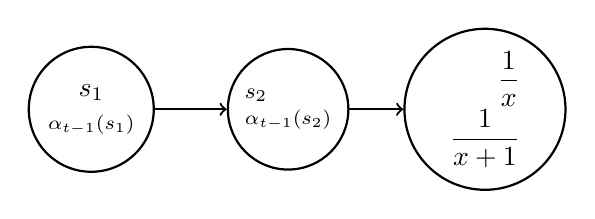
\begin{tikzpicture}
  \node[align=center,circle,draw,thick] (a) at (0,0)
    {$s_1$\\{\scriptsize$\alpha_{t-1}(s_1)$}};
  \node[align=left,circle,draw,thick,font=\footnotesize] (b) at (2.5,0)
    {$s_2$\\{\scriptsize$\alpha_{t-1}(s_2)$}};
  \node[align=right,circle,draw,thick] (c) at (5,0)
    {$\dfrac{1}{x}$\\$\dfrac{1}{x+1}$};
  \draw[->,thick] (a) -- (b);
  \draw[->,thick] (b) -- (c);
\end{tikzpicture}
\end{document}
